\subsection{Input Constrained MPC - Closed Loop Simulation}
In this section the input constrained MPC is simulated on both the linear and non-linear system. For this simulation, the tuning is set to $Q=100$ and $S=0.01$. The constraints is set to 
\begin{equation}
    u_{min}=0\qquad u_{max}=450\qquad \Delta u_{min}=-10\qquad \Delta u_{max}=10
\end{equation}
It should be noticed that the values shown in the plot is absolute values.
\begin{figure}[H]
    \centering
    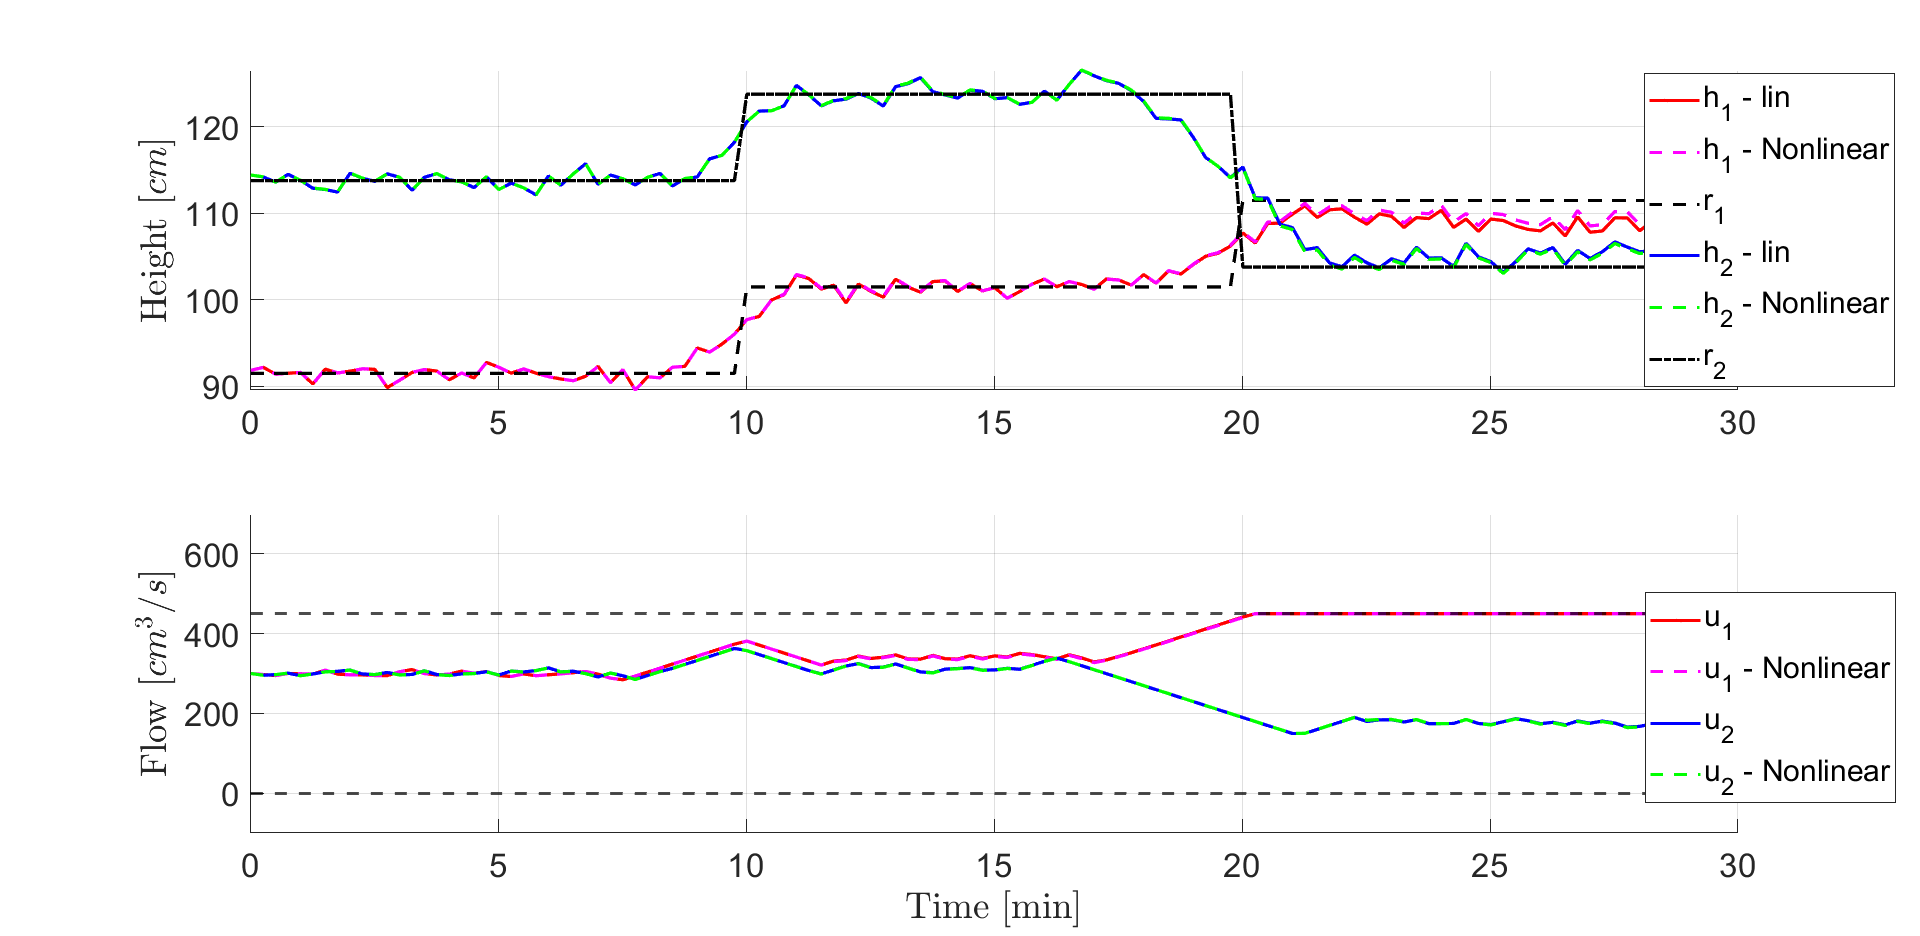
\includegraphics[width=1\textwidth]{Figures/Pr10.2_Input_con_MPC.png}
    \caption{Input constrained MPC - Simulation on linear and non-linear model}
    %\label{fig:Kalman_stoc_state_step}
\end{figure}
As for the unconstrained MPC, the deviation between the linear and the non-linear system is very small. In the case of input constrained MPC, the settling time (in case of step changes in the reference) is longer which is intuitive when the inputs are constrained. It is also seen that the MPC try to regulate earlier (in relation to at which time the reference occurs). In case the constraints on $\Delta u$ was lower, the regulation will begin earlier.
It can be seen that the input 1 is reaching its maximum limit, which causes the reference in tank 1 to be unreachable (however very close). 